\section{Experimento 5} 
El circuito empleado en el experimento anterior funciona como un modulador de
amplitud, aprovechando la zona no lineal de segundo orden (cuadrática) presente en la curva
V-I del diodo. Este comportamiento es buscado.
Sin embargo, también existen no linealidades de orden superior que producen la aparición de
los productos de intermodulación (IMD). El más relevante suele ser el de tercer
orden. En este experimento se busca determinar el rechazo a la IMD de tercer orden del
circuito modulador.

Para poder ver este efecto se debe configurar los generadores de señales de manera que en un principio las señales sean de misma amplitud y frecuencia.
Luego se debe retocar la frecuencia de los generadores hasta que las señales queden equidistantes del pico de máxima sintonía y la separación entre ambas sea de 2KHz aproximadamente

Obteniendo la siguiente figura en el osciloscopio:
\begin{figure}[H]
    \centering
    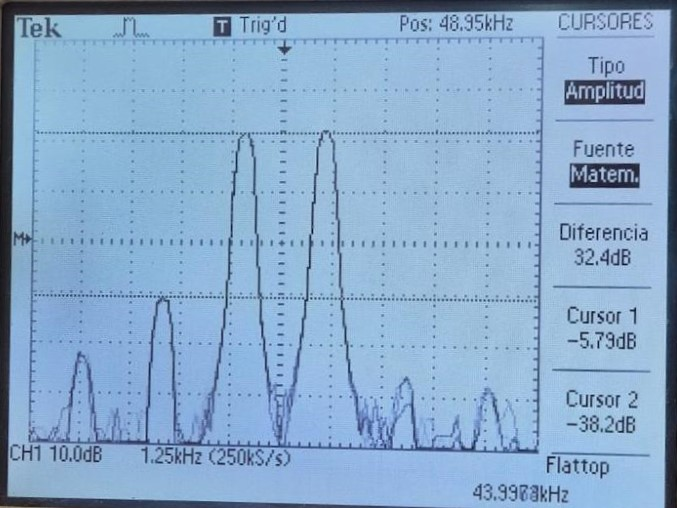
\includegraphics[width=0.4\textwidth]{images/image8.jpg}
    \caption{Señal }
\end{figure}

De donde se pueden registrar los siguientes valores:
\begin{center}
\begin{tabular}{@{}c@{}}
f1:
\underline{\hspace{0.2cm}$48\,\mathrm{kHz}$\hspace{0.2cm}}
f2. :
\underline{\hspace{0.2cm}$50\,\mathrm{kHz}$\hspace{0.2cm}}
\\[0.25cm]
2f1-f2. (Dif.):
\underline{\hspace{0.2cm}$46\,\mathrm{kHz}$\hspace{0.2cm}}
2f2-f1. (Dif.):
\underline{\hspace{0.2cm}$52\,\mathrm{kHz}$\hspace{0.2cm}}
\end{tabular}
\end{center}
\vspace{0.5cm}
Las componentes 2f1-f2, 2f2-f1 son los productos de IMD de tercer orden, y la diferencia
en dB entre las mismas y f1, f2 se denomina Rechazo de IMD de 3er orden:
\vspace{0.5cm}

\begin{center}
\begin{tabular}{@{}c@{\hspace{0.7cm}}c@{}}
$\Delta(\mathrm{dB})_{2f_1-f_2}$:
\underline{\hspace{0.2cm}$48\,\mathrm{kHz}$\hspace{0.2cm}}
&
$\Delta(\mathrm{dB})_{2f_2-f_1}$:
\underline{\hspace{0.2cm}$50\,\mathrm{kHz}$\hspace{0.2cm}}
\end{tabular}
\end{center}